%\section{Genomics}
%Genomics is a wide area of study focusing on the genomes of organisms
%from all varieties of life. A genome is a sequence of characters that
%contains the fundamental set of `rules' used to create what we know as
%life. One can think of a genome as a set of instructions that our
%cells use in order to complete the tasks that make us function. A
%genome is comprised of tightly bundled sequences of DNA, which are
%stored in the nucleus of cells. These bundles of DNA contain sections
%known as genes, which can be thought of as the tools described by the
%set of instructions. These tools carry out a vast number of processes
%ranging from no known function at all to genes that are key in
%protecting against diseases cancer. Genomes can vary widely in size,
%ranging from small bacterial genomes of roughly 4 Mb up to
%approximately 149000 Mb. Piecing together genomes provides numerous
%opportunities to understand other `omics' within cells, such as
%proteomics, metabolomics, transcriptomics and epidemics.

This chapter provides a brief background on \textit{Trichoderma} and gene prediction tools, providing context for this research. Section~\ref{lit:evolution} discusses the evolutionary mechanisms that may have led to the increased production of secondary metabolites in \textit{Trichoderma} species, such as horizontal gene transfer, gene duplication, and transposable elements. Section~\ref{lit:novel-genomes} discusses the novel \textit{Trichoderma} genomes that were sequenced and assembled as part of this work, and how they relate to the research questions. Section~\ref{lit:similarity-searches} discusses the structure of eukaryotic genes as well as a background of gene finding tools and methods, while Section~\ref{lit:secondary-metabolites} provides an overview of secondary metabolites and their importance in \textit{Trichoderma} species. Finally, Section~\ref{lit:comp-motiv} provides an overview of comparative studies of gene prediction tools in \textit{Trichoderma} species, and how this work aims to fill the gap in literature.

\section{\textit{Trichoderma} Species and their Features}\label{lit:features}

\textit{Trichoderma} species are a group of fungi in the \textit{Sordariaceae} family and are found in a wide variety of soils, being well-known for their use in biomanufacturing
of cellulases and hemicellulases and are also known for their roles as non-toxic,
avirulent, opportunistic plant symbionts~\cite{woo2023a, kubicek2019a}. 
Many of these features of \textit{Trichoderma}
can be attributed to the large number of secondary metabolites
produced by these fungi, which are used to interact with plants and other organisms in the soil~\cite{Mukherjee2012}. \textit{Trichoderma} species differ in the number of secondary metabolites they produce, with some species producing more than others~\cite{Mukherjee2012}. This variation in secondary metabolite production is of great interest to researchers, as it can provide insight into how these fungi can confer benefits to plants, and how they can be used in agriculture and industry. In addition, the study of secondary metabolites in \textit{Trichoderma} species can help us better understand
the evolutionary processes that have shaped \textit{Trichoderma} species over time.

There are many mechanisms that organisms may leverage that result in gain or loss of gene function, and ultimately the evolution of a species. One well-studied mechanism is that of horizontal gene transfer (HGT), which is the process of acquiring genetic material from another organism, rather than through inheritance from a parent organism~\cite{goncalves2024}. HGT is a common mechanism in bacteria, but it has also been observed in fungi, including \textit{Trichoderma} species~\cite{goncalves2024}. Another mechanism of interest is the duplication of genes, which can result in the production of more than one copy of a gene, leading to increased expression of that gene~\cite{goncalves2024}. This is particularly relevant in the case of secondary metabolite production, as many \textit{Trichoderma} species have been shown to have multiple copies of genes involved in secondary metabolite production~\cite{Mukherjee2012}. Lastly, transposable elements (TEs) are another mechanism of interest, as they can insert themselves into the genome and disrupt or enhance the expression of genes~\cite{goncalves2024}. TEs have been shown to play a role in the evolution of \textit{Trichoderma} species, particularly in the case of secondary metabolite production~\cite{goncalves2024}. 

Interestingly, both HGT and TEs tend to present themselves in regions where GC content differs from the rest of the genome~\cite{goncalves2024}. Abnormal GC content is also associated with other genomic features, such as centromeres~\cite{plohl2014a} and repetitive regions~\cite{winter2018}, both of which may have an effect on the production of secondary metabolites in \textit{Trichoderma} species. As a result, it is important to consider the GC content of a genome when studying \textit{Trichoderma} species, which forms the basis of the Research Question~\ref{rq:anomalous-sequence-content}. Some studies have shown that \textit{Trichoderma} species contain very few if any transposable elements, which is unusual for fungi~\cite{kubicek2011}. It is hypothesized that TEs were lost in \textit{Trichoderma} due to repeat induced point mutations (RIP), which is a process that occurs in fungi where TEs are silenced and eventually lost from the genome~\cite{kubicek2011}. Genes responsible for RIP mutations also tend to target GC nucleotide pairs, converting them to AT nucleotides, which explains the low GC content observed in some regions of \textit{Trichoderma} genomes~\cite{goncalves2024}. These conversions usually occur when a C nucleotide is adjacent to a downstream A nucleotide.

%One common theory for the increase in secondary metabolites is that \textit%{Trichoderma} initially evolved as a parasite or saprotroph of plants, due to their abundant production of cellulases and plant wall degrading enzymes~\cite{kubicek2019a}. In addition to saprotrophy, \textit{Trichoderma} species are also mycoparasitic, feeding on other Ascomycete and closely related fungal species~\cite{Druzhinina2018}. As a result, it is hypothesized that the elevated production of secondary metabolites in \textit{Trichoderma} arose from the constant change and competition for resources in the environments in which they evolved.~\cite{Mukherjee2012}. While many studies have been conducted on the mechanisms behind fungal evolutionary processes, the process of horizontal gene transfer (HGT), is of particular interest in the case of \textit{Trichoderma}~\cite{goncalves2024}.

Given the proximity of \textit{Trichoderma} species to other fungi, bacteria, and plants in soils, it is possible that \textit{Trichoderma} species acquired genes which are involved in response to antagonistic or sympathetic intercellular interactions from other organisms. While difficult to prove, studies have shown that HGT events have occurred in a number of fungal species~\cite{fitzpatrick2012}. It is also important to note that some \textit{Trichoderma} species have higher numbers of genes involved in secondary metabolite production than others, indicating an evolutionary divergence, making comparative analysis of \textit{Trichoderma} species and strains a useful tool for understanding the mechanisms behind secondary metabolite production~\cite{Mukherjee2012}.

\section{Novel \textit{Trichoderma} Genomes}\label{lit:novel-genomes}

Recently, two strains of \textit{Trichoderma}
have been identified in the prairie regions of Alberta and
Saskatchewan. These two strains, named Tsth20 and DC1, have been found
to have beneficial properties when used as an inoculant for plants in soils. Tsth20 has been classified into the \textit{Trichoderma harzianum} group, and may act as a bioremediation tool in soils contaminated with hydrocarbon content. DC1, while not yet classified, is believed to confer salt and drought tolerance to plants in dry, salty soils. While bioremediation and resistance to drought tolerance has been investigated in other strains of
\textit{Trichoderma}~\cite{senizza2023}, the study of new strains is still useful in the effort of discovering unique mechanisms used by \textit{Trichoderma}. Little is known about these strains, so DC1 and Tsth20 were sequenced at the Global Institute for Food Security in an initial attempt to better understand the mechanisms at work in these genomes. While this research does not explicitly identify genomic elements related to the beneficial properties of these genomes, it may serve as a foundation for future research of \textit{Trichoderma}. The assembly of these genomes come as a result of Research Question~\ref{rq:assembly-results}.

\section{Evolutionary Landscape of \textit{Trichoderma}}\label{lit:evolution}

The evolutionary landscape of \textit{Trichoderma} species is an important aspect of this work. DC1 and Tsth20 have not yet been classified into a specific \textit{Trichoderma} species, although Tsth20 has been tentatively declared a \textit{harzianum}, and further understanding of their evolutionary relationships to other \textit{Trichoderma} species may help explain how DC1 and Tsth20 originated. 
Figure~\ref{fig:phylogeny} shows the phylogenetic relationships among selected \textit{Trichoderma} species as well as the outgroup \textit{Fusarium graminearum}. The tree was constructed using cursory alignments of the \textit{Rpb2} gene, which is a commonly used gene for phylogenetic analysis in fungi~\cite{an2022}. Representative \textit{Rpb2} proteins from the various fungal species were extracted from the NCBI resource for fungal orthologs, while representative \textit{Rpb2} proteins from DC1 and Tsth20 were identified from the results generated later on in this work. \textit{Trichoderma} species separate into a number of distinct clades, and these clades can vary between studies as evidenced by the low confidence in placement of \textit{T. atroviride} and \textit{T. gamsii}. Lack of confidence in evolutionary relationships is not uncommon in \textit{Trichoderma} species, and is likely due to the high levels of horizontal gene transfer and gene duplication that have occurred in these species~\cite{goncalves2024}. This makes \textit{Trichoderma} species interesting to study but difficult to classify. 

\begin{figure}
    \centering
    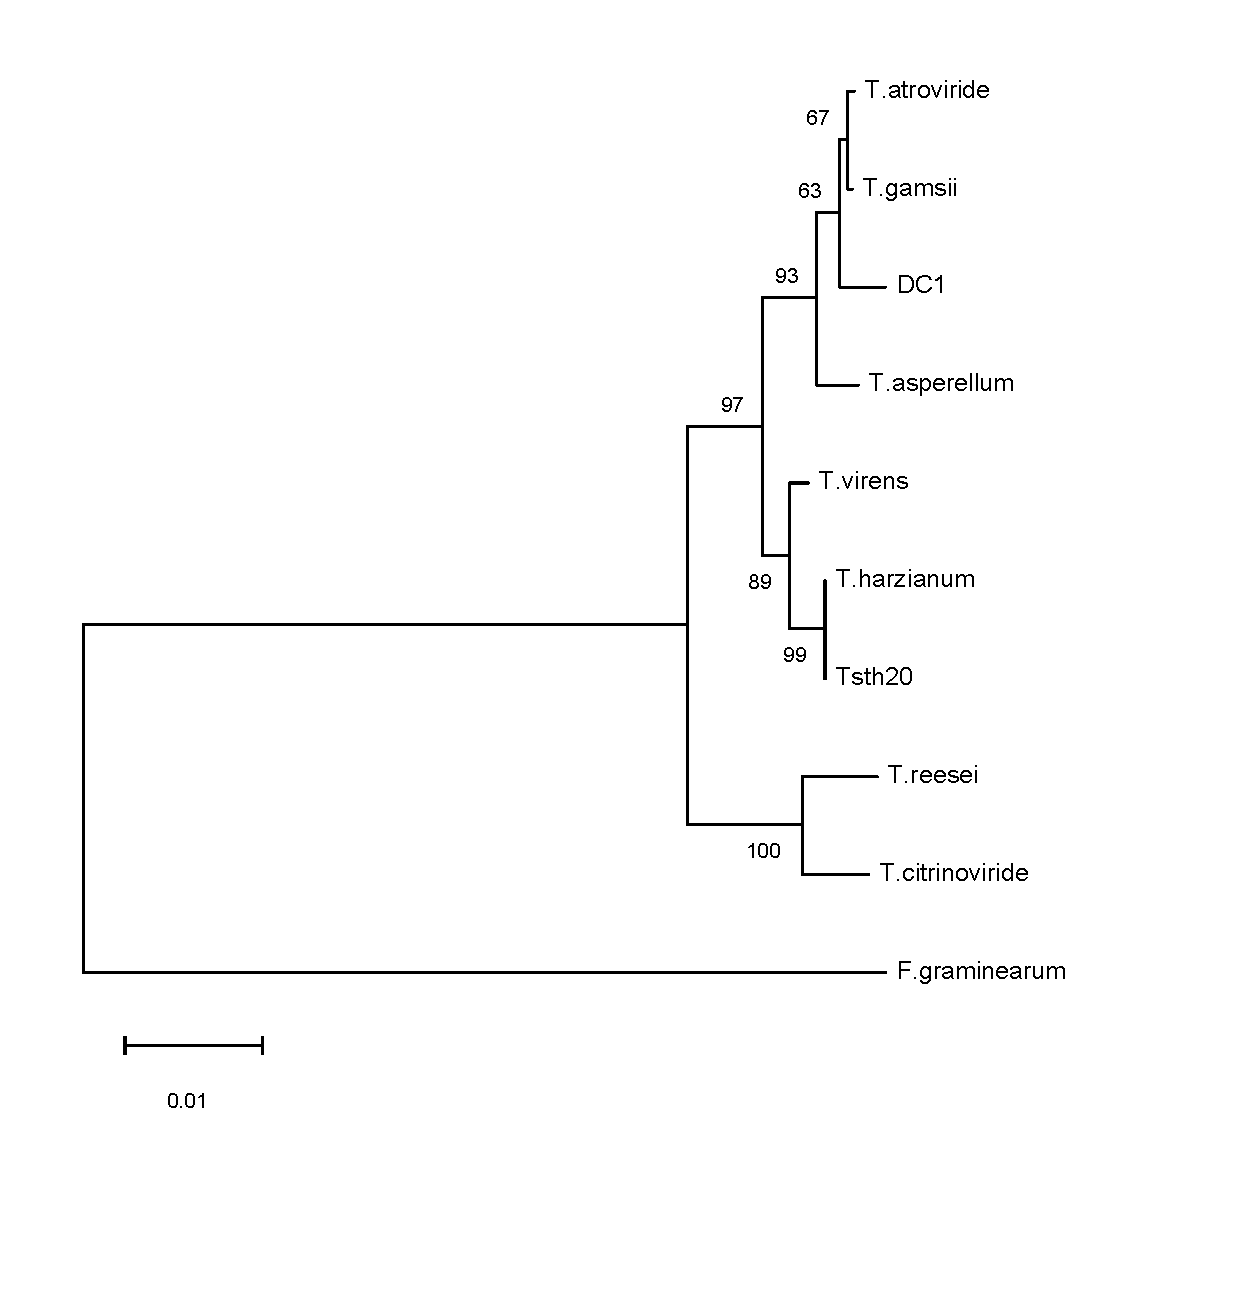
\includegraphics[width=\textwidth]{figures/trichoderma-phylogeny-few-outgroups.pdf}
    \caption[\textit{Trichoderma} Phylogenetic tree]{Phylogenetic tree illustrating relationships among selected \textit{Trichoderma} species based on multiple sequence alignments of \textit{Rpb2}. Evolutionary history was inferred using the Neighbour-Joining method~\cite{Saitou1987}. The optimal tree with the sum of branch lengths = 0.146 is shown. The percentage of replicate trees in which the associated taxa clustered together in the bootstrap test (1000 replicates) are shown next to the branches~\cite{Felsenstein1985}. The tree is drawn to scale, with branch lengths in the same units as those of the evolutionary distances used to infer the phylogenetic tree. An example branch of length 0.01 is shown.}\label{fig:phylogeny}
\end{figure}

Phylogeny is also important when selecting genomes for comparative analysis of bioinformatics tools. Some tools may vary in their performance depending on the nature of the genome they are applied to, making a heterogeneous selection of genomes important for understanding the performance of the tools in different contexts. In this work, we selected three well-studied \textit{Trichoderma} species, \textit{T. reesei, T. harzianum}, and \textit{T. virens}, which are all commonly used in research and industry, but are relatively distant from each other evolutionarily according to more detailed studies~\cite{an2022}. 

%\section{Environmental Stress}

%Crop resistance to environmental stressors is a necessity for crop
%health and overall crop yields. Current popular methods for crop
%protection involve the use of pesticides and genetically modified
%organisms, which can be expensive and potentially politically dividing
%in the case of GMOs~\cite{doi:10.1080/10408390600762696}. In addition,
%crops suffer when soils are not sufficient for crop growth and
%health. Soil insufficiencies can result in drought stress as well as
%nutrient stress, leading to poor overall yields.

\section{Gene Predictions and Complementing Similarity Searches}\label{lit:similarity-searches}

Gene prediction methods are generally based on the idea that genes can be
identified by searching for patterns in a sequence, which match an expected gene structure or model. These gene structures begin from a $5'$ start codon, continue through a series of exons and introns, and end with a $3'$ stop codon~\cite{loftus2003a}. Flanking the gene structure are promoter regions, which are typically found upstream of the start codon, and untranslated regions (UTRs), which are found both upstream of the $5'$ start codon and downstream of the $3'$ stop codon. Promoter regions are important for the regulation of gene expression, while UTRs are important for the stability and translation of the mRNA transcribed by the gene~\cite{loftus2003a}. Sequences are translated from the $5'$ start codon through to the $3'$ stop codon, splicing together exons and ignoring introns. An example of a eukaryotic gene structure is shown in Figure~\ref{fig:gene-structure}.

\begin{figure}[ht]
    \centering
    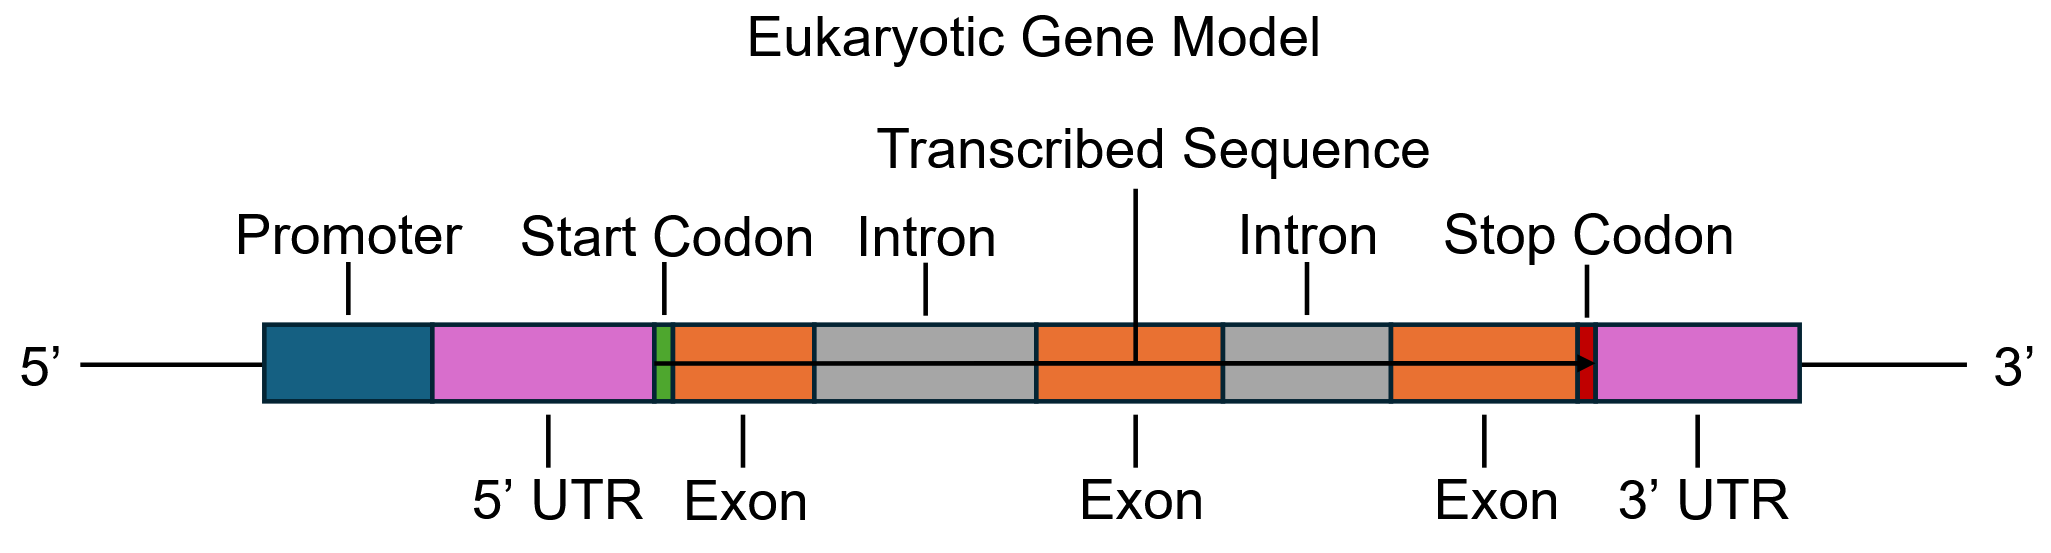
\includegraphics[width=0.8\textwidth]{figures/gene-model-fig-msc.png}
    \caption[Generic gene model]{Example of a eukaryotic gene structure, showing a promoter region (blue), the $5'$ and $3'$ UTRs (purple), start codon (green), exons (orange), and introns (gray). The directed arrow indicates the direction of transcription. }\label{fig:gene-structure}
\end{figure}

Gene prediction methods vary in their approach, but they generally fall into two categories: \textit{ab initio} methods and evidence-based methods~\cite{ejigu2020a}. \textit{Ab initio} methods rely on the identification of patterns in the sequence that match an expected gene structure, while evidence-based methods use prior information such as RNAseq data, expressed sequence tags (ESTs), and expressed protein sequences to identify genes within a new genome~\cite{ejigu2020a}. Gene prediction methods can also vary in their ability to identify different components of a gene, such as the promoter region, UTRs, and introns. Some methods may only identify the coding sequence (CDS) of a gene, while others may also identify the promoter region and UTRs~\cite{ejigu2020a}. Making things more complicated, different gene prediction tools may predict different combinations of exons and introns for a gene, and some tools may even predict multiple combinations of exons and introns, leading to multiple transcripts for the same gene. As a result, different transcripts may produce different proteins, which can significantly impact function~\cite{ejigu2020a}. Given the already complex nature of secondary metabolites, it is important to consider the impact of variability in gene prediction methods, especially in the case of \textit{Trichoderma} species and their secondary metabolite production. This consideration is one of the main motivators behind this research, and forms the basis of Research Question~\ref{identify-regions}.

As mentioned earlier, gene finding tools generally fall into one of two categories: \textit{ab initio} and evidence-based. \textit{Ab initio} methods are often used when no prior information is available, and include tools such as GeneMark~\cite{borodovsky2011a}, GenScan~\cite{burge1997}, and GlimmerHMM~\cite{majoros2004}. Evidence-based methods are used when prior information is available~\cite{ejigu2020a}, and include tools such as BLAST and other alignment tools to identify sequences in the genome that are similar to known sequences. More recently, hybrid tools have been developed that combine both \textit{ab initio} methods and evidence from RNAseq data, ESTs, and protein sequences to identify genes in a genome~\cite{ejigu2020a}. These hybrid tools are often more accurate than either \textit{ab initio} or evidence-based methods alone, as they can take advantage of the strengths of both approaches. Some examples of hybrid tools include AUGUSTUS~\cite{stanke2003}, Braker2~\cite{bruna2021a}, and MAKER~\cite{cantarel2008}. GeneMark and Braker2 were selected as tools for comparison in this work as they are both widely used in the field, with high citation counts of over 2000 and 1600 respectively on individual papers, and also represent an \textit{ab initio} method and a hybrid method, respectively. Braker2 was a particularly interesting option, as it combines GeneMark with AUGUSTUS as part of its workflow. Purely evidence-based gene prediction methods were not selected for this work, as they require prior information such as RNAseq data, which was not available for DC1 and Tsth20. The NCBI RefSeq annotations for the additional \textit{Trichoderma} assemblies were also used as a point of comparison as they are generated using a combination of \textit{ab initio} and evidence-based methods, and are considered to be high-quality annotations. RefSeq annotations may be generated by the NCBI Eukaryotic Genome Annotation Pipeline~\cite{zotero-item-367} or by other sources as long as the annotation is approved by NCBI for the organism of interest. To simplify discussion surrounding the NCBI representative annotations, they will be referred to as RefSeq throughout the rest of this work.

While the basic structure of a gene may be present in a sequence, that does not mean that the gene codes for a functional protein, or in the case of secondary metabolites, a component that helps produce them. To assess potential function of a gene product, gene prediction methods are often used in conjunction with similarity searches, which compare the predicted genes to known genes in other organisms to identify potential functions, and serve as a form of validation for the predicted genes~\cite{loftus2003a}. 
Similarity searches can come in several different forms, such as BLAST searches, which compare the predicted genes to a database of known proteins, or InterProScan, which compares the predicted genes to a database of known protein domains and binding motifs~\cite{loftus2003a}. These similarity searches can provide additional information about the predicted genes, such as potential functions, and can also help to validate the predicted genes by comparing them to known genes in other organisms. Similarity searches can also be used to evaluate the completeness of the predicted genes. One example would be comparing predicted genes to a set of conserved single-copy orthologs expected in fungal genomes, such as those provided by BUSCO~\cite{manni2021a}. Together, these methods can provide a more complete picture of the gene predictions and their potential functions, which allows us to better understand the performance of these gene finders in the context of fungal genomes. This forms the basis of Research Questions~\ref{rq:interproscan},~\ref{rq:tblastn}, and~\ref{rq:busco-completeness}.

\section{Secondary Metabolites}\label{lit:secondary-metabolites}

While cellular products essential to an organism's viability are
of great interest, there are a vast number of cellular products that while not
essential, still provide great benefit to the
organism and may be necessary for survival in some situations~\cite{Craney2013, Mukherjee2012}. These other cellular products are known
 as secondary metabolites, and they are involved in several roles ranging 
 from cellular signalling to antibiotic activity, making them a frequent 
 subject of study in pharmaceutical research. Enzymes that produce 
 secondary metabolites are comprised of non-ribosomal peptide synthetases 
 (NRPS) and polyketide synthetases (PKS), which synthesize amino acids and 
 other basic enzymatic building blocks into proteins~\cite{komaki2020}. 
 Genes encoding the NRPSs and PKSs responsible for production of secondary 
 metabolites are often found in clusters within a genome, but their 
 products remain unknown~\cite{Mukherjee2012}. 
 
 The study of these products is difficult as the genes encoding the modules that make up NRPSs and PKSs are not expressed under normal laboratory conditions~\cite{Mukherjee2012}. The NRPSs and PKSs that have been studied
 have been shown to be large enzymatic structures containing several 
 functional modules, each responsible for a specific step in the synthesis 
 of a protein~\cite{Mukherjee2012}. Studying these complicated mechanisms and their genes requires as close to a complete set of gene predictions as possible, as the absence of one gene encoding a module could affect the entire protein complex. This concept of completeness of gene predictions is explored in Research Question~\ref{rq:busco-completeness}. 
 In addition, gene predictions can be processed further with tools such as antiSMASH, which can identify secondary metabolite biosynthetic gene clusters (BGCs) in a genome~\cite{blin2023}. Comparison of predicted genes with known secondary metabolite BGCs can provide insight into completeness of the predicted genes with a specific focus on secondary metabolite production. This work is not covered in this thesis, but is worth noting for context as it is a common approach in the field of secondary metabolite research.

 Another interesting feature of NRPSs and PKSs is the length of the genes encoding them, which can be quite long, often exceeding 10,000 base pairs in length~\cite{komaki2020}. Examining the outputs of gene prediction tools can provide insight into the lengths of predicted genes, and whether the tools are able to capture the full length of these large genes. This topic serves as the basis for Research Question~\ref{rq:gene-lengths}.  

 %Given the modular nature of NRPSs and PKSs, one can assume that many genes %are responsible for the production of secondary metabolites. Thus, it is %important that methods used for the identification of genes involved in %secondary metabolite production are able to identify as many of those genes %as possible. Failure to identify these genes may result in an incomplete %understanding of the secondary metabolite production process, and may also %result in the loss of potential targets for further research. With this in %mind, it is important to consider the methods used for identification of %genes in a genome, as the methods used can have a significant impact on the %results, forming the basis of Research Questions ~\ref{rq:number-of-features} %and ~\ref{rq:gene-lengths}. 

\section{Gene Prediction Tools in Fungi}\label{lit:comp-motiv}

With the biological context laid out, we can now turn our attention to the computational aspect of this work. Many \textit{Trichoderma} species have been assembled and annotated in the past, mostly for the purpose of understanding the mechanisms behind secondary metabolite production~\cite{Mukherjee2012}. Gene predictions in this context are typically compared against sequences from other organisms to derive functional information, and to validate the predicted genes~\cite{loftus2003a}. In contrast, very few studies have been conducted comparing gene prediction tools in fungal genomes, and even fewer have been conducted in \textit{Trichoderma} species. This is surprising, given the large number of gene prediction tools available, and the fact that many of them are used in the field of fungal genomics~\cite{ejigu2020a}. Comparisons of gene prediction tools are common when new tools are released, but these comparisons are often limited to a few tools, and tend to be focused on achieving higher counts of interesting genes, rather than comparing the results in a biological context~\cite{min2017}. Complicating the matter further, the quality of genome sequences available may vary, making evaluation of different gene prediction tools difficult when working with multiple genomes and lesser-studied fungal species with low quality assemblies. Given the gap in literature regarding comparative analysis of gene prediction tools in \textit{Trichoderma} species, and the availability of the novel DC1 and Tsth20 genomes, this work aims to fill that gap by comparing the outputs of several gene prediction tools on these two genomes along with three other frequently studied \textit{Trichoderma} species. 

Another pitfall of existing literature is that many studies compare tools only against a reference annotation, such as the RefSeq annotations for some organisms. However, these reference datasets are not always available, may not be representative of the genome being studied, and may be incomplete. In addition, it is helpful to compare the outputs of gene prediction tools against each other, as this can provide insight into the strengths and weaknesses of each tool relative to one another. For these reasons, this work aims to compare outputs of gene prediction tools in an all-to-all manner, rather than an all-to-one manner.

Finally, most studies comparing gene prediction tools also include more technical metrics of gene finders, such ease of installation and use, run times, memory usage, and other computational metrics. These metrics can be important when selecting a tool, as users may be limited by the computational resources available to them, or may require results in a timely manner. Additionally, not all users are comfortable with command line tools, and may prefer a tool that is easy to use, and includes useful documentation.  

%\section{Genome Assembly}

%Sequence assembly has been a long-standing problem in the field of
%bioinformatics~\cite{nagarajan2013a}. Determining the correct order and
%combination of smaller subsequences into an accurate complete sequence
%assembly is computationally difficult in terms of compute resources
%such as memory, CPU cycles and storage required for input
%sequences~\cite{nagarajan2013a}. In addition to these difficulties,
%there can be other issues encountered during assembly due to the
%nature of the data or genomes themselves, such as low quality base
%calls for long read data, which is not necessarily the case today, or
%the inherent content of genomes themselves using repetitive regions as
%an example. Insufficient data may result in short, fragmented
%assemblies, depending on the size of the genomes, while sequence data
%that is not long enough can fail to fully capture repetitive regions
%in an assembly. A wide range of assembly tools have been developed
%with their own unique approaches to the genome assembly problem, so it
%is important to use an appropriate assembler for the task at hand, and
%also important to evaluate the assembly thoroughly.

%Genome assembly tools generally approach the assembly problem using a
%graph-based approach. The most common graph-based approach is the de
%Bruijn graph assembly~\cite{compeau2011a}. A graph in this context, is
%set of nodes (\textit{k}-mers from sequences) connected by edges
%(overlaps between \textit{k}-mers). Traversing through this graph
%results in longer subsequences that ultimately result in a set of
%sequences referred to as an assembly. In the early years of long read
%sequence data, sequencing platforms encountered difficulties producing
%consistently high scores for base calls when sequencing. To combat
%this, some assembly workflows may also include a polishing or
%correction step once the initial assembly is completed in which high
%quality short read sequences are used as supplemental information to
%correct low quality regions in the assembly. These low quality base
%calls are typically not present in modern long read sequencing
%approaches as the methodology and quality of calls have improved
%drastically. While the polishing step is arguably unnecessary in
%modern assemblies, the polishing programs remain available should
%researchers be interested in applying additional reads for polishing.

%One approach to aid in the previously mentioned issue of assembly
%correctness is to use a combination of long and short reads in what is
%known as a hybrid assembly. Combining both highly accurate short reads
%with deep coverage along with less accurate but much longer reads can
%produce high quality genome assemblies that capture long repetitive
%regions. Hybrid assembly approaches have been shown to produce high
%quality assemblies in a wide variety of organisms as the combine long
%read data with short data to produce assemblies that properly
%represent long repetitive regions with additionally high quality
%Illumina sequences for correction. Once assembled, the sequences must
%also be evaluated with measures such as N50, L50, coverage, average
%contig length and total assembled length to ensure that the genomes
%are well assembled, at least based on these
%metrics~\cite{nagarajan2013a}. Following appropriate assembly protocols
%is essential to the further success of a project as downstream
%processing such as annotation depends on a high-quality assembly.

%\section{Identification of Anomalous Genomic regions}
%One important aspect of interest when assembling any form of sequence
%is GC content or percent GC of the assembled sequence. Large regions
%of anomalous GC content may be of interest to researchers as they may
%contain repetitive regions and unique features responsible for traits
%specific to the organism in question.



%\section{Gene Finding Methods}
%Gene finding (or gene annotation) has been a long standing
%computational problem in bioinformatics, which concerns itself with
%identifying potential genes within assemblies based on patterns or
%pre-existing experimental evidence considered by the gene finding
%program. This process is critical for unraveling and understanding the
%complex processes occurring in all forms of life. In a general sense,
%gene finding programs operate by searching for patters or indicators
%showing that a gene of feature may be present. The most basic
%indicators being start and stop codons, with splice sites in
%between should the sequence match the applied model. The results
%produced by gene finding tools can vary considerably for a number of
%reasons, including quality of the assembly, the intrinsic model used
%by the gene finder, filtering criteria, and even the nature of the
%organism and assembly itself. Given the broad applications, choice of
%gene finding tools, and the variability of assemblies being
%considered, it is important that we gain a deeper understanding of
%these tools prior to putting them to use.

%There are two common methods for gene finding, those methods being
%\textit{ab initio} methods, where programs search for patterns and
%gene structures, and similarity or evidence-based searches, which use
%prior information such as RNAseq data, expressed sequence tags and
%expressed protein sequences to identify genes within a new
%genome~\cite{ejigu2020a}. Complicating the process more is the
%introduction of introns and alternative splicing in eukaryotes, making
%it possible for one gene to have several possible transcripts at the
%same locus. An example of an \textit{ab initio} method would be
%GeneMark-ES~\cite{borodovsky2011a}, while an evidence based tool
%would be Braker2~\cite{bruna2021a}.
%\textit{Ab initio} gene finders typically predict genes using a Hidden
%Markov Model (HMM)~\cite{ejigu2020a}. These predictions are based on
%`signals' or features associated with a gene, such as the usual start,
%stop, exon and intron portions of a gene as well as upstream promoter
%sequences and more. In this case, these signals would be considered
%states in the terminology associated with HMMs. Gene finders wish to
%predict these states based on observations, or sequences presented to
%the model. HMMs in gene finding tools are trained beforehand and then
%applied to a sequence. This means that a gene finding program may not
%be trained in the context of any assembly provided to it, and thus may
%miss genes that are unique to the assembly in question.
%On the other hand, while still relying on HMMs for a `base' set of
%predictions, evidence-based gene finding tools leverage new evidence
%that may be outside the scope of the pre-existing
%model~\cite{Keller2011}.  As an example, an evidence-based model would
%be useful in a situation where you are interested in annotating a new
%assembly for a non-model organism. The addition of experimental data
%provides context specific to your assembly of interest while still
%retaining the predictions from existing HMM models.

%There are also other aspects of gene finding tools that are important
%to consider. These include features such as whether or not the gene
%finders find non-coding RNAs, annotation of 5' and 3' UTR regions, and
%in the case of ab-initio methods, the assumptions made by the
%underlying models used for gene finding. These features and others can
%influence a user's decision on which gene finding tool to consider and
%will complicate comparative analysis of multiple gene finding
%tools. (citation needed somewhere in here)

%\section{Repeat Identification and Masking}
%Repeat identification within assembled genomes is a problem that needs
%to be considered during the genome annotation process. Regions with
%long repeats can have a significant impact on genome assembly as well
%as gene finding due to the limitation of short reads used in some
%assemblies~\cite{Treangen2011}. Short reads may be unable to bridge or
%cover entire repeat regions within a genome, so it is important to
%consider the use of long reads from technologies such as Nanopore or
%PacBio\texttrademark ~\cite{Rhoads2015} to provide a complete picture of
%these regions when pursuing a new genome assembly project. It is also
%possible for repetitive regions to contain genes as well, making for
%an interesting investigation in regards to \textit{Trichoderma}, as
%fungal genomes have been shown to contain many repeat regions with a
%high concentration of A and T
%nucleotides~\cite{winter2018}. Once these repetitive
%regions have been identified, the genome could be masked as a method
%to mark these regions for downstream processing if desired, as these
%regions may be poorly assembled and may result in found genes that do
%not truly exist in those regions. However, this may not be as common
%today, as repetitive regions have been shown to contain genes as
%well~\cite{Slotkin2018}. This may affect the gene finding process
%described later and may be an interesting topic to look into
%considering the large number of available gene finding programs.

%\section{Centromere Identification}
%A centromere is a region of a chromosome that is crucial for the
%proper cell division. These regions are the main anchor for
%microtubules, which are fibers that attach to centromeres to separate
%chromosomes during both mitosis and meiosis. Centromeres are critical
%to the survival of an organism, with malfunctions in the process of
%cell division usually resulting in potential disease and fatal
%outcomes~\cite{plohl2014a}. Centromeric sequences can be comprised of
%several different genetic components, with repetitive regions being
%the most prevalent in the forms of satellite DNA and transposable
%elements. In addition to centromeric regions, there are flanking
%pericentric regions with their own properties, including potential
%candidates for small-interfering RNAs~\cite{plohl2014a}. Identification
%and consideration of centromeric regions may prove useful when
%comparing the outputs of gene finding tools, as the underlying
%properties and structure of the genetic sequence differ in comparison
%to typical coding regions of DNA.

%\section{Sequencing}
%Sequencing data is a pivotal form of data used in nearly all
%applications of Bioinformatics. To understand the processes used by
%organisms for survival, we must have an initial set of data points to
%work with. These sequences, referred to as reads after sequencing, are
%the foundation for solving problems ranging from taxonomical
%classification to the understanding or complex biological functions
%like signaling pathways. Reads may come in a variety of forms and
%formats depending on the desired application.

%\section{Whole Genome Shotgun Sequencing}
%Whole Genome Shotgun sequencing (WGS), is a method to produce a large
%number of genomic sequences from a sample of interest for the purpose
%of genome assembly. This is form of sequencing is quite common as it is
%has a wide variety of applications in research~~\cite{Adams2008}. WGS
%involves slicing up genomic DNA into smaller segments. These small
%segments are then processed further resulting in a set of physical
%molecules that can be supplied to a compatible sequencing platform of
%which there are a variety. Modern sequencing platforms are comprised
%of next generation sequencing (NGS) and 3rd generation sequencing
%approaches.

%\section{Next Generation Sequencing - Illumina}
%Illumina\texttrademark ~~\cite{Bennett2004} sequencing is one of the
%most popular NGS platforms currently available. Illumina sequencing
%produces a very large number of high quality short reads, typically
%between 75 and 250 base pairs in length. Sequencing libraries can be
%prepared to produce reads solely from one end of a sequence fragment
%(single-end) or both ends (paired-end). Advantages of paired end
%sequences are the additional context provided by the paired sequence
%on the opposite end of the fragment. This context is leveraged by read
%processing tools to identify features such as repetitive regions and
%genomic rearrangements, which can be significant in downstream
%analyses. Illumina sequence libraries are generated by first
%fragmenting the DNA samples, amplifying them via PCR, ligating
%adapters that allow the sequence to bind to the sequencing plate, and
%finally identifying each fragment's sequence of nucleotides using
%fluorescent-labeled nucleotides that bind to the
%fragments~~\cite{Goodwin2016}.

%\section{3rd Generation Sequencing - Nanopore}

%Nanopore\texttrademark ~~\cite{Wang2021} sequencing data is relatively
%recent approach to sequencing projects. While Illumina reads are
%short, Nanopore reads are much larger, ranging from 10Kb to 300Kb
%depending on the approach used. Long reads are beneficial due to their
%ability to bridge the gaps between difficult to assemble regions when
%performing sequence assembly. An example of a difficult to assemble
%region would be a region with a high repeat content, where a large
%number of small repeats may be collapsed during the assembly process,
%resulting in an assembly that does not represent the true nature of
%the sequence being studied~~\cite{Marx2023}. While Nanopore was
%previously known for having lower quality base calls when compared to
%Illumina, that is no longer the case at this time. Nanopore sequencing
%works by passing long segments of genetic sequence through a membrane
%bound protein and measuring changes in electrical current, which is
%characteristic of the nucleotide at a given position.

%\section{RefSeq}

%First, we will briefly discuss the RefSeq annotation process. RefSeq
%annotation is only applied to data that is submitted to NCBI. The evRefSeq Eukaryotic Genome Annotation Pipeline~\cite{NCBI2024} is a
%genome annotation process developed and maintained by NCBI. The pipeline is not directly publicly available to public users, and
%requires submission of data to NCBI. Once data is submitted to NCBI,
%the RefSeq annotation pipeline may be applied upon request only if the
%genome is the highest quality assembly for the species in question or
%if the genome is of significant interest to the scientific community,
%limiting reach of the annotation process to many users. The pipeline
%supplies existing RNAseq, CDS and protein sequences to NCBI's in-house
%gene prediction tool Gnomon, which produces trained models for gene
%prediction. While the tools used for alignment and processing of
%supporting sequence information are listed, the inner workings of
%Gnomon are not well documented, at least from the public perspective,
%and I was unable to find Gnomon in any compilable or executable form
%during my search. Recreation of the RefSeq pipeline would prove
%extremely challenging if not impossible without supporting
%information. Run times for this pipeline are difficult to determine
%due to the hidden nature of the pipeline, unknown compute resources
%and varying quantities of data used. The evfSeq annotation process
%produces comprehensive outputs, including CDS sequences, translated
%CDS, RNA from genomic sequences, proteins, feature counts and tables,
%and finally GFF and GTF formatted annotation files for these features.

%\section{InterProScan}
%The outputs from gene finding tools are a set of potential genes that
%fit the model used by each tool. While they are considered genes, the
%use of the word gene is used in a very loose sense, in that these
%genes may or may not be functional or match any existing gene
%sequences from previous research. Typically, to confirm the
%'correctness' of predicted genes, the outputs from a given tool are
%used in a sequence similarity search against a reference set of genes
%or a large database comprised of multiple organisms. This approach is
%straightforward, but can introduce bias from database choice and also
%allows for vague or loose matches, depending on the parameters used
%and the interpretation of the results. Another approach is to use
%InterProScan, which is a tool used for functional annotation of
%proteins using evidence from a variety of databases
%~\cite{10.1093/nar/gkac993}. The presence of some form of functional
%domain or annotated structure in a predicted gene sequence is
%reasonable evidence for the existence of a predicted gene. This
%approach also avoids the problems associated with similarity-based
%approaches.


%\section{File Formats}

%\subsection{FASTA}
%One of the most popular formats for sequences of DNA, RNA and amino
%acids is the FASTA format. The evSTA format consists of one or more
%entries containing two or more lines. The first line of an entry is
%the ID line, which must begin with a greater-than (\textgreater)
%character, followed by an ID and any other pertinent information for
%the following sequence. The greater-than character is the indicator
%that a new sequence has begun. The following line(s) contain the
%actual sequenced nucleotides or amino acids, which can be contained on
%one line or split across many lines. An example of multiple FASTA
%entries are shown in figure~~\ref{fig:fasta-example}.

%\begin{figure}
%  \centering
%  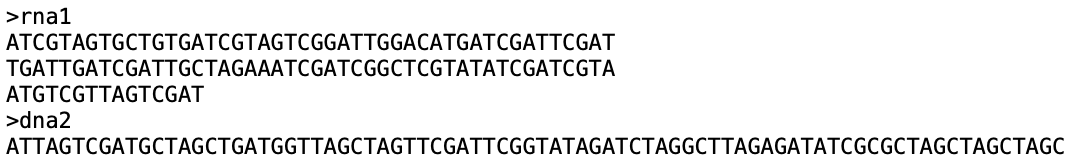
\includegraphics[width=0.8\textwidth]{figures/fasta-example.png}
%  \caption{Example of two FASTA sequence entries. One example with
%    sequence characters split across multiple lines, and one showing
%    all sequence characters on the same line.}
%  \label{fig:fasta-example}
%\end{figure}

%\subsection{FASTQ}
%Another popular sequencing format is the FASTQ format. This format is
%very similar to the FASTA format but with the addition of two more
%lines per sequence entry and a change to the character indicating the
%beginning of a new sequence entry. An example of a FASTQ entry is
%shown in figure~~\ref{fig:fastq-example}. In FASTQ formatted entries,
%the greater-than (\textgreater) character is swapped with the at (@)
%character. The evs for the sequence also follow a specific format,
%which provide information about the sequencing run and flowcell that
%the read was sequenced on. This information can then be traced back to
%the sequencing experiment in the case that there were errors or
%anomalies in the output from the experiment. Following the ID is the
%string of base calls. The third line in a FASTQ entry is a plus (+)
%character, which indicates that the sequences character line has
%finished. Following the plus character is another sequence of
%characters, this time indicating the quality of basecall for the
%corresponding nucleotide base calls in the second line. The quality
%information included in FASTQ files are used to assess the quality of
%a sequencing run and extensively used in downstream processing steps,
%most notably in alignments.

%\begin{figure}
%  \centering
%  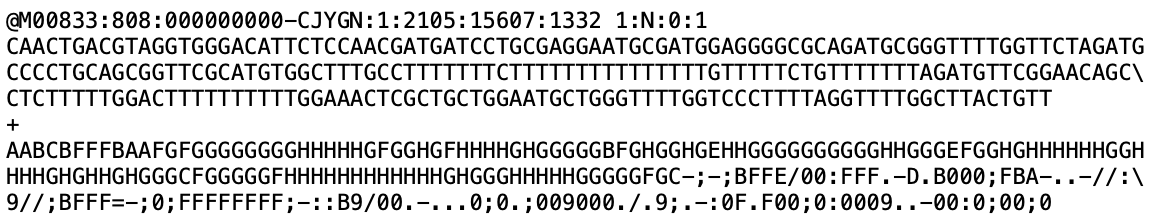
\includegraphics[width=0.8\textwidth]{figures/fastq-example.png}
%  \caption{Example of the four lines in a FASTQ entry.}
%  \label{fig:fastq-example}
%\end{figure}

%\subsection{General Feature Format - GFF}
%General feature format (GFF) is a popular format for storing
%information about features relative to a position on an genetic
%sequence, and comprises a large portion of annotation results from
%this work. These features can be whatever the user desires, as long as
%the feature entry follows the required GFF guidelines. Relative to a
%reference sequence, each GFF entry contains the following
%tab-delimited columns: sequence ID, source, feature type, start
%position, end position, score, strand, phase, and a semi-colon
%delimited list of attributes. GFF files are widely supported across
%bioinformatics tools, making them highly versatile while also
%remaining relatively simple in nature but also allowing for storage of
%more complicated items via the attributes column. One significant
%usage of GFF files is in visualization of features against the
%reference sequence from which they were derived. Most genome viewers
%(or browsers) support GFF files as input, allowing intuitive
%visualization of many features when overlaid on a reference
%sequence. An example of a GFF entry can be seen in
%figure~~\ref{fig:gff-example}.

%\begin{figure}
%  \centering
%  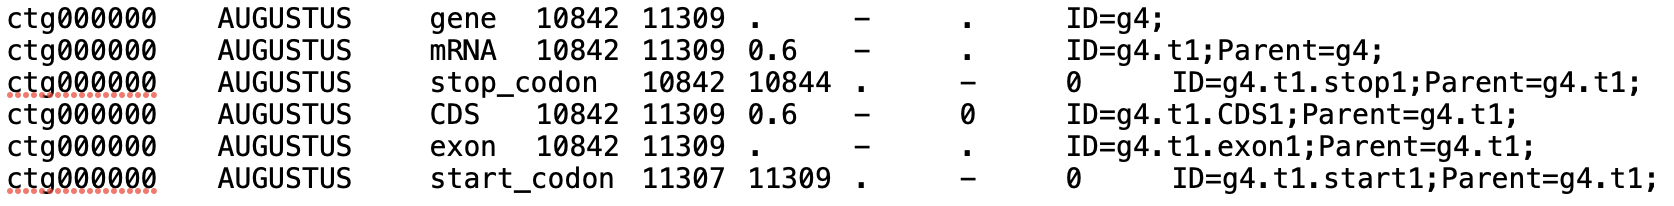
\includegraphics[width=0.8\textwidth]{figures/gff-example.png}
%  \caption{An example of GFF entries for a single gene.}
%  \label{fig:gff-example}
%\end{figure}

%\section{BLAST and tblastn}
%The basic local alignment search tool (BLAST)~\ref{Altschul1990} has
%been a popular tool in the bioinformatics space, used to align
%biological sequences and measure their similarity. The original blast
%program was developed for alignment of nucleotide sequences, but other
%blast tools have been developed as well. One of these tools is tblastn
%which was developed to align reverse-translated protein sequences to
%another nucleotide sequence. To align the protein sequences, the query
%nucleotide sequences are translated in all six reading frames and then
%aligned to the proteins.  Tblastn is particularly useful for
%identifying functional or conserved proteins in	a nucleotide sequence.

%\section{BUSCO}
%The benchmarking Universal Single-Copy Orthologs
%(BUSCO)~\ref{10.1093/bioinformatics/btv351} tool was developed to
%evaluate assemblies and subsequent annotations from the perspective of
%gene orthology. As genomes diverge evolutionarily, it is expected that
%some genes will be conserved as they are required for basic
%function. The BUSCO (Benchmarking Universal Single-Copy Orthologs)
%tool and datasets were developed to assess completeness of an
%annotation in comparison to evolutionarily conserved genes.
